\section {Implementação de um servidor NTP}

%\subsection{Introdução}

\begin{frame}
\frametitle{Implementação de um servidor NTP}
\framesubtitle{Introdução}

\begin{itemize}
  \item Problema: rede de controle do \textit{Sirius} será isolada. Como
  sincronizar todos os \textit{logs} e \textit{timestamps}?
  \item Receptadores GPS fornecem:
  \begin{itemize}
    \item Horário no formato UTC.
    \item Pulsos 1PPS (\textit{pulse-per-second}), indicando o início de um novo
    segundo e precisão na ordem de nanosegundos.
  \end{itemize}
  \item NTP + Hora UTC + 1PPS = servidor de \textit{stratum 1}
  
  \item 3 modelos comprados:
  \begin{itemize}
    \item \textit{Ultimate GPS Breakout} da \textit{Adafruit}.
    \item \textit{GPS Click} da \textit{MikroElektronika}. 
    \item \textit{CAM M8Q} da \textit{ublox}.
  \end{itemize} 
\end{itemize}

\end{frame}

\begin{frame}
\frametitle{Implementação de um servidor NTP}
\framesubtitle{Instalação}


\begin{itemize}
  \item \textit{Ultimate GPS Breakout}:
  \begin{figure}[h]
    \centering
    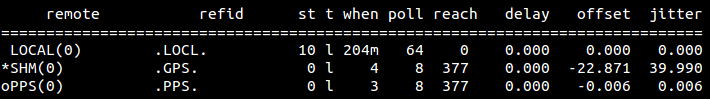
\includegraphics[width=0.80\textwidth]{image/adafruit_GPS}
    \label{img:adafruit} 
  \end{figure} 
  \item \textit{GPS Click}:
  \begin{figure}[h]
    \centering
    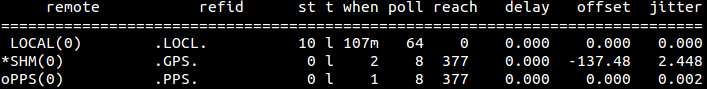
\includegraphics[width=0.80\textwidth]{image/mikroe}
    \label{img:mikroe} 
  \end{figure} 
  \item Comparação:
  \begin{figure}[h!]
    \centering
    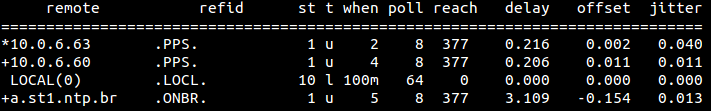
\includegraphics[width=0.80\textwidth]{image/cliente-ntp}
    \label{img:cliente_ntp} 
\end{figure} 
\end{itemize}

\end{frame}

%\subsection{Implementação de variáveis EPICS}
 
\begin{frame}
\frametitle{Implementação de um servidor NTP}
\framesubtitle{Variáves EPICS - \textit{daemon NTPD}}

\begin{itemize}
  \item Variáveis EPICS definidas para o \textit{daemon NTPD} :
  
  \vspace{12pt}
  
	\begin{itemize}
	\item  \textcolor{red}{\textbf{\texttt{NTP:Leap}}: indicação de um eventual
	\textit{leap second} pendente.}
	\item \texttt{NTP:Stratum}: \textit{stratum} do servidor.
	\item \texttt{NTP:Refid}: ID de referência da fonte de sincronismo.
	\item \textcolor{red}{\textbf{\texttt{NTP:Offset}}: \textit{offset} entre o
	relógio do sistema e da fonte.}
	\item \textcolor{red}{\textbf{\texttt{NTP:Jitter}}: desvio padrão das medidas
	\textit{offset} mais recentes.}
	\item \texttt{NTP:Precision}: precisão do \textit{clock} do sistema em \textit{log2}.
	\item \texttt{NTP:Srcadr}: endereço IP do servidor. 			
	\item \texttt{NTP:Version}: versão e data de compilação.
	\item \textcolor{red}{\textbf{\texttt{NTP:Timestamp}}: diferença, em segundos,
	entre a data atual do servidor e a \textit{unix epoch} (1 de Janeiro de 1970).}
	\end{itemize}	    
\end{itemize}	

\end{frame}

\begin{frame}
\frametitle{Implementação de um servidor NTP}
\framesubtitle{Variáves EPICS - \textit{daemon GPSD}}

\begin{itemize}
  \item Variáveis EPICS definidas para o \textit{daemon GPSD} :
  \vspace{12pt}
	\begin{itemize}
	\item \textcolor{red}{\textbf{\texttt{GPS:Fix}}: indicação do tipo de
	\textit{fix} (\textit{no fix}, 2D ou 3D \textit{fix}).}
	\item \texttt{GPS:Latitude}: latitude medida pelo GPS.
	\item \texttt{GPS:Longitude}: longitude medida pelo GPS.
	\item \texttt{GPS:Altitude}: altitude medida pelo GPS.
	\item \textcolor{red}{\textbf{\texttt{GPS:Sattelites}}: \textit{string}
	contendo a identificação dos satélites usados para o \textit{fix}.}
	\item \textcolor{red}{\textbf{\texttt{GPS:Timestamp}}: \textit{timestamp}
	fornecido, análogo à mesma variável do servidor NTP.}
	\end{itemize}	    
\end{itemize}
\end{frame}

\begin{frame}
\frametitle{Implementação de um servidor NTP}
\framesubtitle{Interface gráfica} 
\begin{figure}[h]
    \centering
    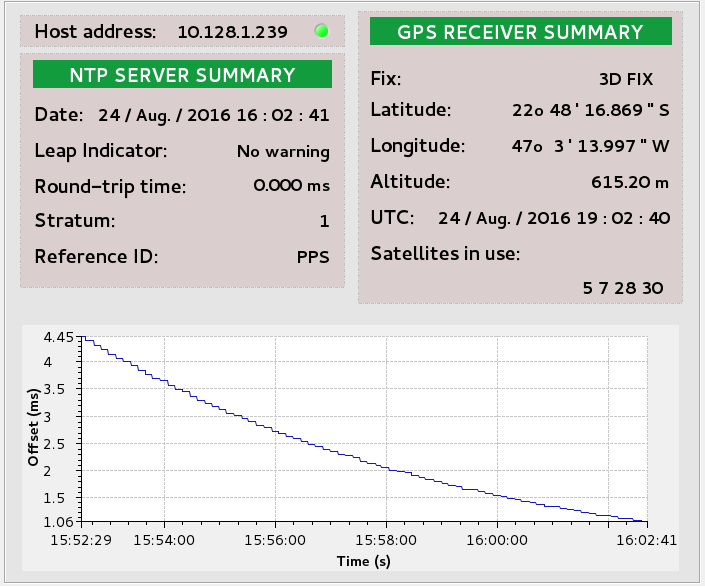
\includegraphics[scale=0.26]{image/epics-opi-ntpgps}
    \caption {Interface construída para visualização das
    \textit{PVs}.}
    \label{img:ntp-opi} 
\end{figure} 

\end{frame}